\section{Auswertung}

\subsection{Überprüfung der Bragg-Bedingung}
Zur Verifzierung der Bragg-Bedingung ist in Abbildung \ref{fig:Bragg} das Spektrum der Kupfer-Röntgenröhre mit den Werten in Tabelle 1 dargestellt.

\begin{figure}[H]
    \centering
    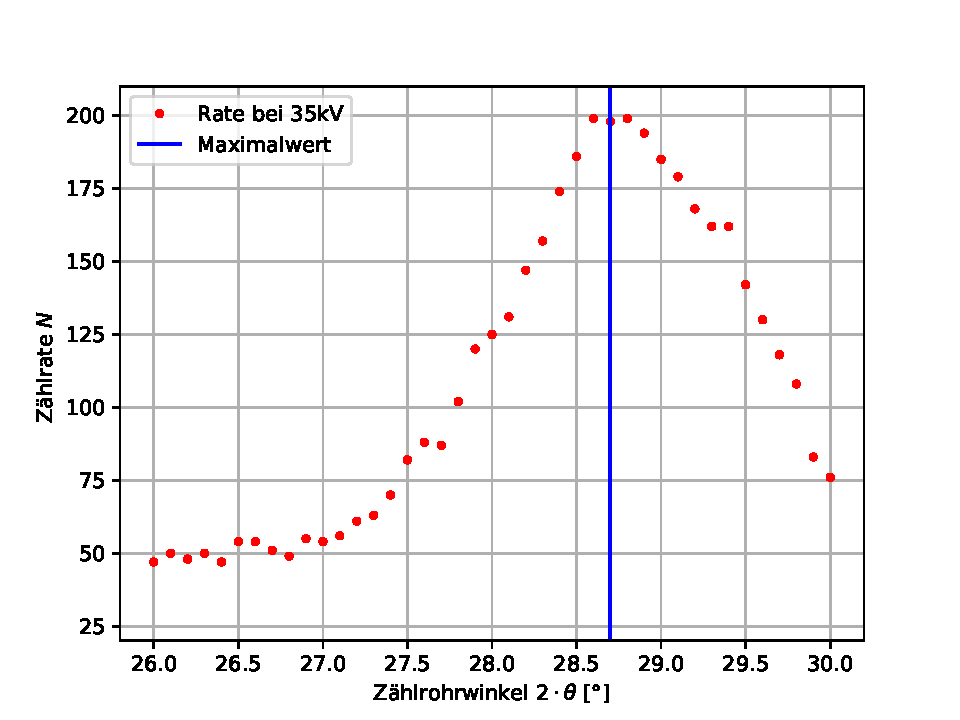
\includegraphics[height=8cm]{Auswertung/Bragg.pdf}
    \caption{Spektrum der Kupfer-Röntgenröhre.}
    \label{fig:Bragg}
\end{figure}

Dabei liegt das Maximum der Messung bei $2 \; \theta = 28.7°$.
Bei einem eingestellten Kristallwinkel von $\theta_\text{theo} = 14°$ ergibt sich eine Abweichung von $2.5\%$.
Die Bragg-Bedingung lässt sich bei einer so geringen Abweichung als erfüllt ansehen.

\subsection{Das Emissionsspektrum}
In Abbildung \ref{fig:Emission} ist das Emissionspektrum der Röntgenröhre mit den Werten aus Tabelle 1 dargestellt.

\begin{figure}[H]
    \centering
    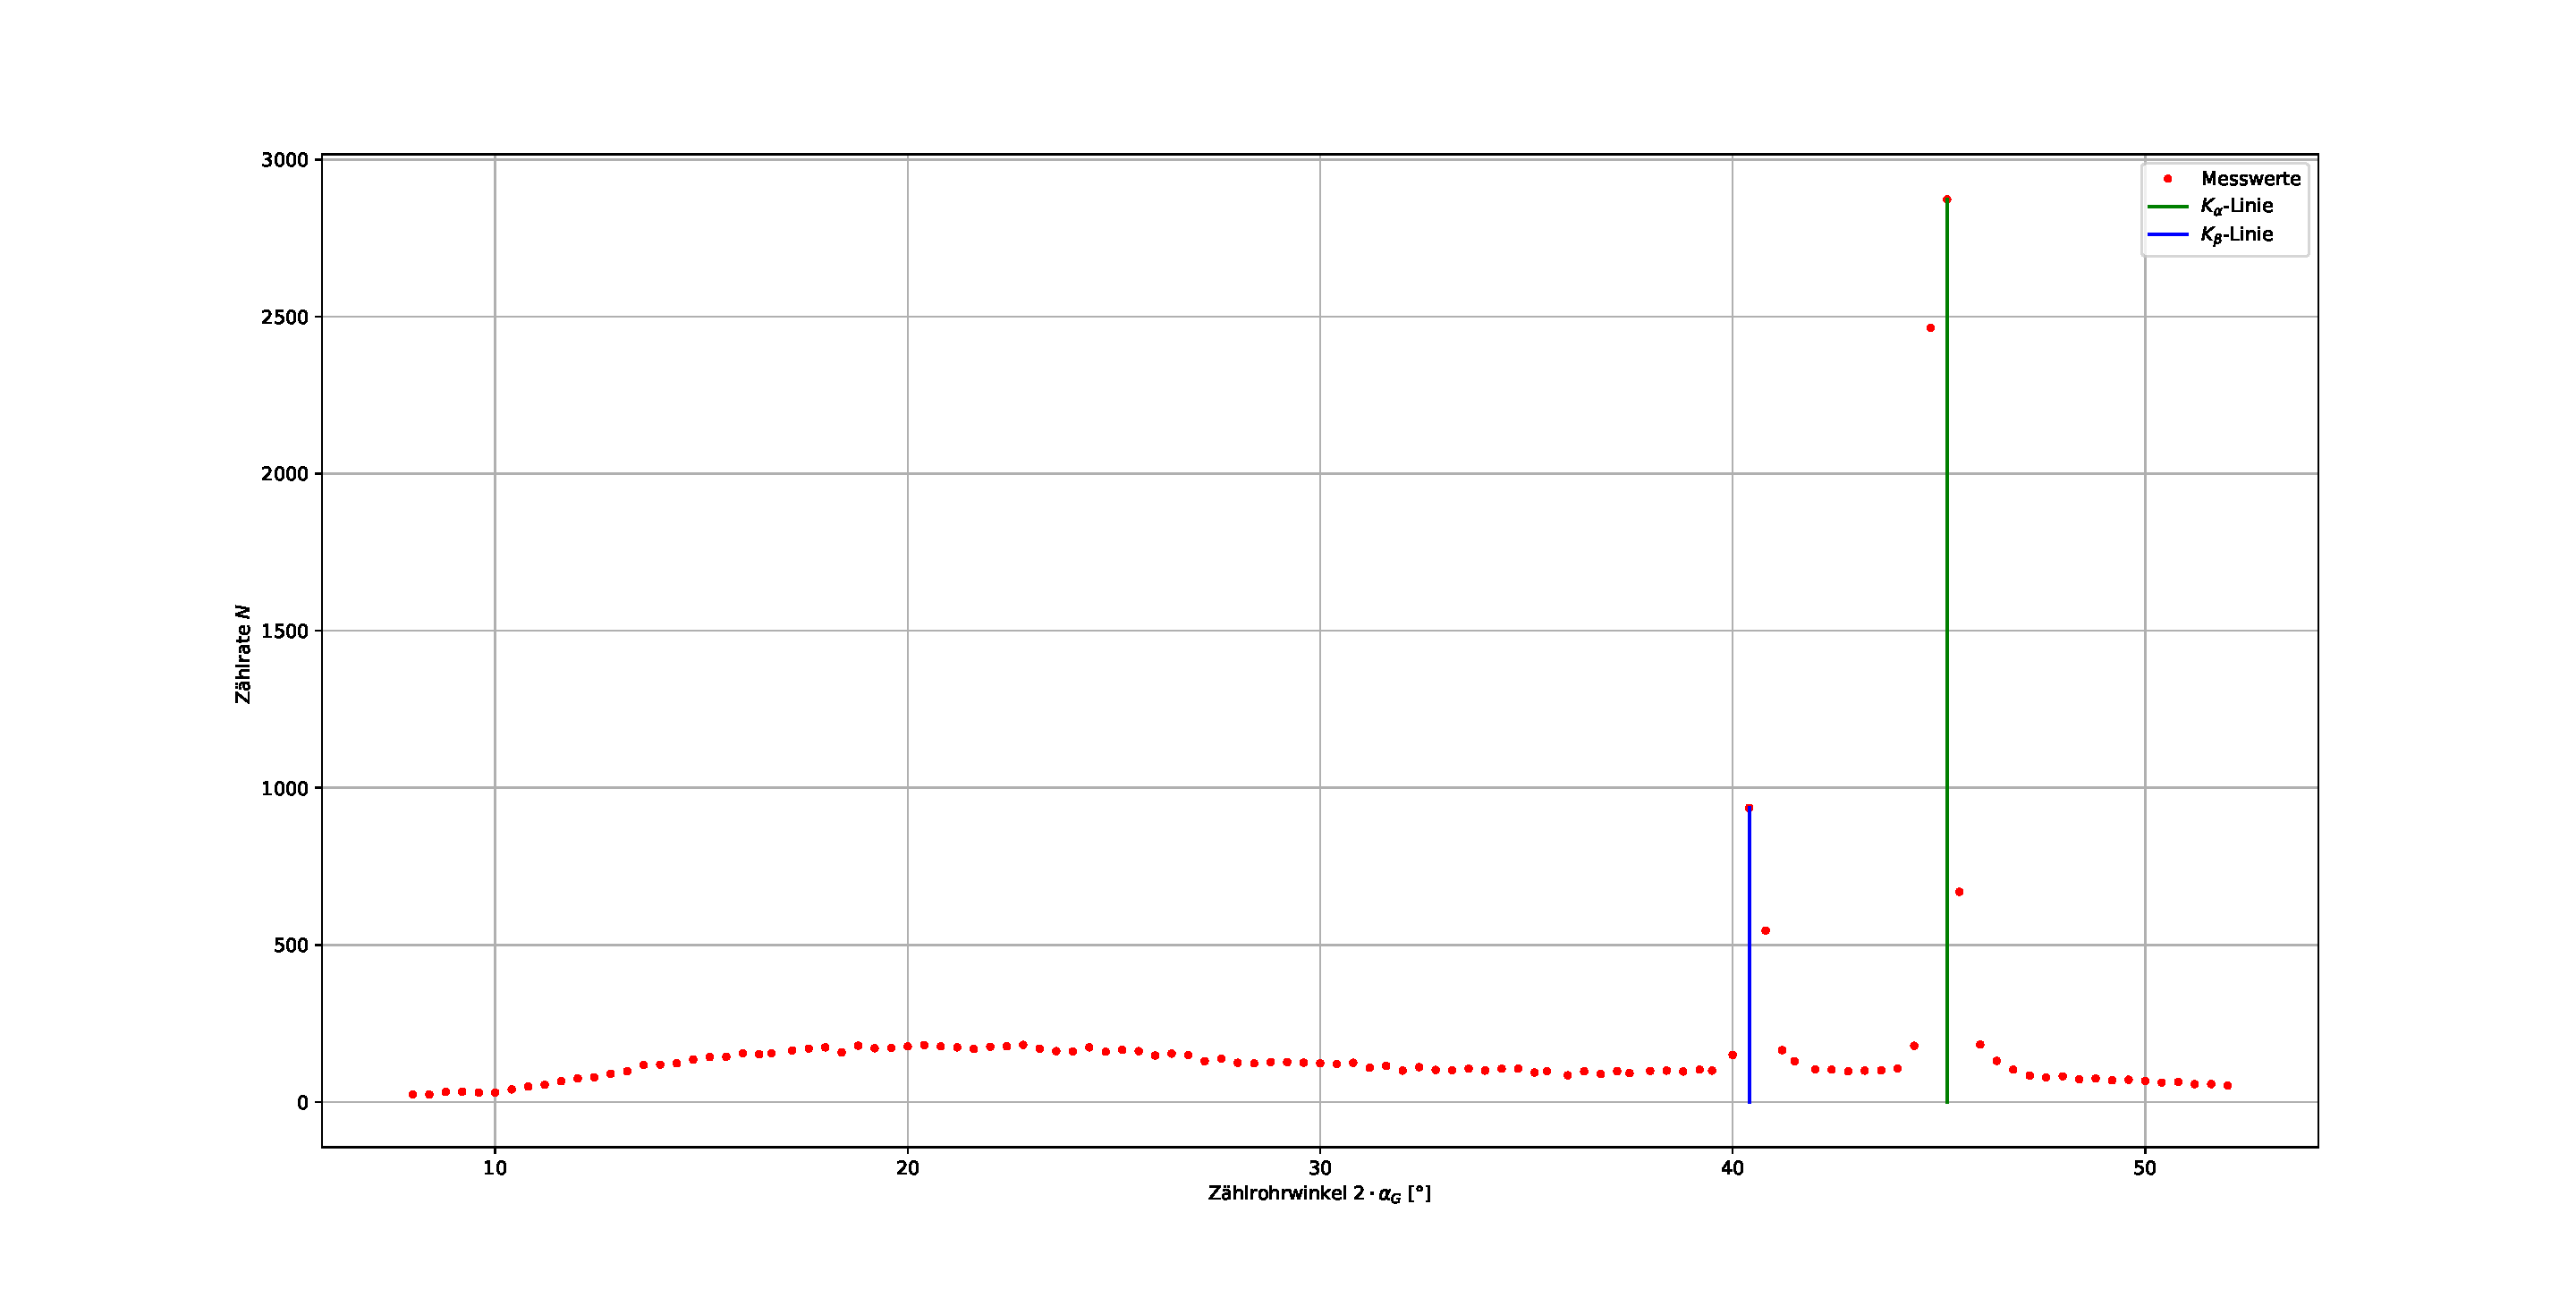
\includegraphics[height=8cm]{Auswertung/Emission.pdf}
    \caption{Emissionspektrum der Kupfer-Röntgenröhre.}
    \label{fig:Emission}
\end{figure}

Dabei beschreibt der kleinere erste Peak die $K_\beta$-Linie und der höhere zweite Peak die $K_\alpha$-Linie.
Der Bereich um die beiden charakteristischen Peaks wird als Bremsberg bezeichnet.
Der Grenzwinkel liegt bei $\theta_\text{Gr} = 5°$ und die daraus resultierende minimale Wellenlänge des Maximums 1. Ordnung ergibt nach Gleichung \ref{eq:5}
\begin{equation}
    \lambda_\text{min} = \SI{35,11}{pm},  \notag
\end{equation}
wobei $d = \SI{201,4}{pm}$ der Abstand der Netzebenen des LiF-Kristalls ist.
Für die daraus resultierende Energie ergibt sich
\begin{equation}
    E_\text{max} = \SI{35,385}{keV}.  \notag
\end{equation}
Bei einer Spannung von $U = \SI{35}{kV}$ lässt sich der theoretische Wert auf $E_\text{max,theo} = \SI{35}{keV}$ bestimmen.
Es ist eine Abweichung von $1,1\%$ festzustellen.

Zur Bestimmung der Halbwertsbreite werden die beiden Punkte der $K_\beta$-Linie und der $K_\alpha$-Linie verwendet, bei der der Maximalwert zur Hälfte abgefallen ist.
Über die lineare Interpolation werden bei der $K_\beta$-Linie die Werte
\begin{equation}
    \theta_1 = \SI{19,892}{°} \qquad \text{und} \qquad \theta_2 = \SI{20,544}{°}  \notag
\end{equation}
bestimmt und damit ergeben sich nach Gleichung \ref{eq:5} Energien von
\begin{equation}
    E_1 = \SI{9,064}{keV} \qquad \text{und} \qquad E_2 = \SI{8,789}{keV}.  \notag
\end{equation}
Dabei ist $\theta_1$ der Winkel vor dem Maximum und $\theta_2$ der Winkel hinter dem Maximum, bei denen die Zählrate der Hälfte des Maximums entspricht.
Für die  $K_\alpha$-Linie ergeben sich Winkel von
\begin{equation}
    \theta_1 = \SI{21,957}{°} \qquad \text{und} \qquad \theta_2 = \SI{22,392}{°}  \notag
\end{equation}
und daraus resultierende Energie von
\begin{equation}
    E_1 = \SI{8,248}{keV}\qquad \text{und} \qquad E_2 = \SI{8,097}{keV}.  \notag
\end{equation}
Die Energiedifferenzen geben die Halbwertsbreiten für die $K_\beta$-Linie und der $K_\alpha$-Linie an und betragen
\begin{equation}
  \Delta E_\beta = \SI{0,275}{keV} \qquad \text{und} \qquad \Delta E_\alpha = \SI{0,151}{keV}.  \notag
\end{equation}
Die Halbwertsbreiten geben dabei das Auflösungsvermögen an.
Das gemittelte Auflösungsvermögen mit dem daraus folgenden Fehler beträgt
\begin{equation}
    \Delta E = \SI{0.213 \pm 0.062}{keV}. \notag
\end{equation}

Zur Bestimmung der Abschirmkonstante wird die Energiedifferenz der Maxima der beiden Linien bestimmt.
Es ergeben sich Winkel und nach Gleichung \ref{eq:5} berechnete Energien für die $K_\beta$-Linie von 
\begin{equation}
  \theta_\beta = \SI{20,1}{°} \qquad \text{und} \qquad E_\beta = \SI{8,93}{keV}  \notag
\end{equation}
und für die $K_\alpha$-Linie
\begin{equation}
  \theta_\alpha = \SI{22,6}{°} \qquad \text{und} \qquad E_\alpha = \SI{8,03}{keV}. \notag
\end{equation}

Nach Gleichung \ref{eq:2} lassen sich die Energien aus den Abschirmkonstanten berechnen und umgekehrt.
Mit der Näherung $E_\beta \approx E_K$ ergibt sich für die $K_\beta$-Linie bzw. für die Abschirmkonstante $\sigma_1$
\begin{equation}
  E_\beta =  R_\infty (z-\sigma_1)^{2}  \iff \sigma_1 = z \pm \sqrt{\frac{E_\beta}{R_\infty}}.  \notag
\end{equation}

Die Energie der $K_\alpha$-Linie bzw. die Abschirmkonstante $\sigma_2$ lassen sich durch Gleichung \ref{eq:2} durch
\begin{equation}
  E_\alpha = R_\infty (z-\sigma_1)^{2} - \frac{1}{4} R_\infty (z-\sigma_2)^{2} \iff \sigma_2 = z \pm 2 \sqrt{(z-\sigma_1)^{2} - \frac{E_\alpha}{R_\infty}}  \notag
\end{equation}
bestimmen.
Für die dritte Abschirmkonstante ergibt sich nach Gleichung \ref{eq:2}
\begin{equation}
    E_\beta = R_\infty (z - \sigma_1)^{2} - \frac{1}{9} R_\infty (z-\sigma_3)^{2} \iff \sigma_3 = z \pm 3 \sqrt{(z-\sigma_1)^{2} - \frac{E_\beta}{R_\infty}}    \notag
\end{equation}
Bei einer Kernladungszahl von $z = 29$ und den berechneten Energien für die beiden charakteristischen Linien ergeben sich Abschirmkonstanten von
\begin{equation}
  \sigma_1 = 3,375  \qquad \text{,} \qquad \sigma_2 = 12,727 \qquad \text{und} \qquad \sigma_3 = 28,545. \notag
\end{equation}


\subsection{Die Absorptionsspektren}
\subsubsection{Galliumabsorber}
Bei der Verwendung von Gallium als Absorber für Röntgenstrahlung wird das Absorptionsspektrum aus Abbildung \ref{fig:gallium} mit den Werten aus Tabelle 2 aufgezeichnet.

\begin{figure}[H]
    \centering
    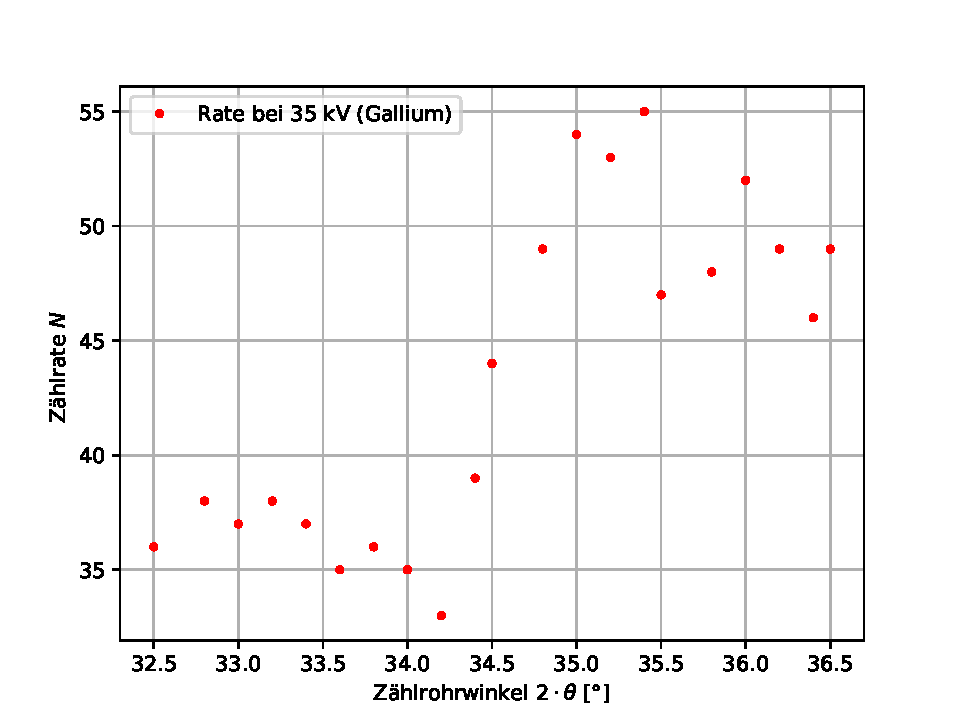
\includegraphics[height=8cm]{Auswertung/Gallium.pdf}
    \caption{Absorptionsspektrum für Gallium.}
    \label{fig:gallium}
\end{figure}

Zur Bestimmung der K-Kante wird der Winkel bei der Hälfte der maximalen Zählrate verwendet.
Für Gallium wird dabei ein Winkel und eine dazugheörige Energie von
\begin{equation}
    \theta = \SI{17.3}{°} \qquad \text{und} \qquad E = \SI{10,372}{keV}  \notag
\end{equation}
bestimmt.
Im Vergleich zu dem theoretisch bestimmten Wert von $E_\text{theo} = \SI{10,380}{keV}$ ergibt sich eine Abweichung von $0,07\%$.
Mittels Gleichung \ref{eq:3} wird die Energie der K-Kante durch
\begin{equation}
    E_\text{$1$,$\frac{1}{2}$} = - R_\infty \left ((z - \sigma_1)^{2} + \frac{1}{4}\alpha^{2}z^{4}\right) \notag
\end{equation}
berechnet, wobei die Quantenzahl $n = 1$ und der Elektronenspin $j = \frac{1}{2}$ sind.
Durch Umformen wird dann die Abschirmkonstante nach
\begin{equation}
    \label{eqn:ab}
    \sigma_1 = z \pm \sqrt{\frac{\alpha^{2}}{4}z^{2} + \frac{E}{R_\infty}} 
\end{equation}
bestimmt.
Die Abschirmkonstante beträgt mit $z = 31$
\begin{equation}
    \sigma_1 = 3,162,   \notag
\end{equation}
wobei der theoretische Wert $\sigma_\text{1,theo} = 3,151$ beträgt und der Wert somit eine Abweichung von $0,35 \%$ hat.


\subsubsection{Zinkabsorber}
Bei der Verwendung von Zink als Absorber für Röntgenstrahlung wird das Absorptionsspektrum aus Abbildung \ref{fig:Zink} mit den Werten aus Tabelle 3 aufgezeichnet.

\begin{figure}[H]
    \centering
    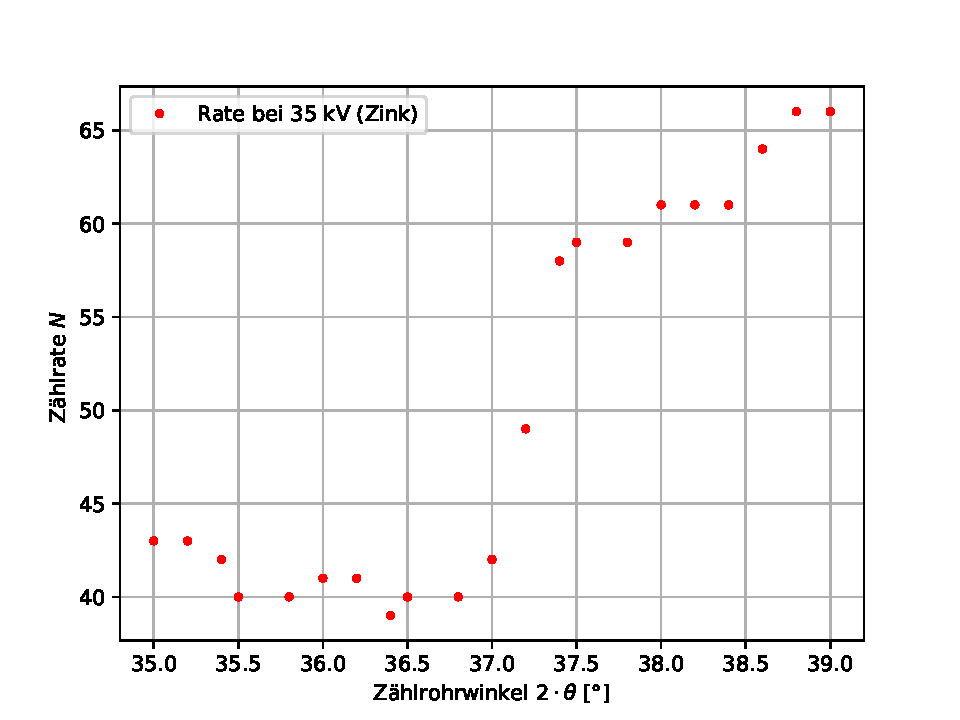
\includegraphics[height=8cm]{Auswertung/Zink.pdf}
    \caption{Absorptionsspektrum für Zink.}
    \label{fig:Zink}
\end{figure}

Zur Bestimmung der K-Kante wird der Winkel bei der Hälfte der maximalen Zählrate verwendet.
Für Gallium wird dabei ein Winkel und eine dazugheörige Energie von
\begin{equation}
    \theta = \SI{18.6}{°} \qquad \text{und} \qquad E = \SI{9,670}{keV}  \notag
\end{equation}
bestimmt.
Im Vergleich zu dem theoretisch bestimmten Wert von $E_\text{theo} = \SI{9,650}{keV}$ ergibt sich eine Abweichung von $0,2\%$.
Mittels Gleichung \ref{eqn:ab} wird die Abschirmkonstante mit $z = 30$
\begin{equation}
    \sigma_1 = 3,134   \notag
\end{equation}
bestimmt, wobei der theoretische Wert $\sigma_\text{1,theo} = 3,560$ beträgt und der Wert somit eine Abweichung von $11,9 \%$ hat.

\subsubsection{Zirkoniumabsorber}
Bei der Verwendung von Zirkonium als Absorber für Röntgenstrahlung wird das Absorptionsspektrum aus Abbildung \ref{fig:Zirkonium} mit den Werten aus Tabelle 4 aufgezeichnet.

\begin{figure}[H]
    \centering
    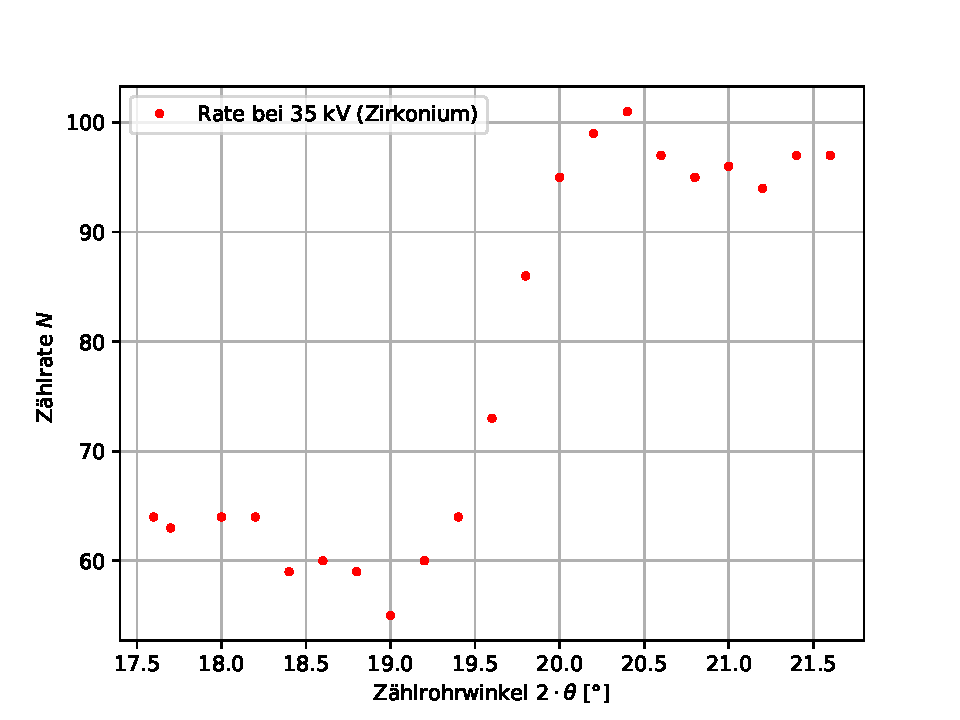
\includegraphics[height=8cm]{Auswertung/Zirkonium.pdf}
    \caption{Absorptionsspektrum für Zirkonium.}
    \label{fig:Zirkonium}
\end{figure}

Zur Bestimmung der K-Kante wird der Winkel bei der Hälfte der maximalen Zählrate verwendet.
Für Gallium wird dabei ein Winkel und eine dazugheörige Energie von
\begin{equation}
    \theta = \SI{9,9}{°} \qquad \text{und} \qquad E = \SI{17,939}{keV}  \notag
\end{equation}
bestimmt.
Im Vergleich zu dem theoretisch bestimmten Wert von $E_\text{theo} = \SI{18,010}{keV}$ ergibt sich eine Abweichung von $0,4\%$.
Mittels Gleichung \ref{eqn:ab} wird die Abschirmkonstante mit $z = 40$
\begin{equation}
    \sigma_1 = 3,215   \notag
\end{equation}
bestimmt, wobei der theoretische Wert $\sigma_\text{1,theo} = 4,080$ beträgt und der Wert somit eine Abweichung von $21,2 \%$ hat.

\subsubsection{Bromabsorber}
Bei der Verwendung von Brom als Absorber für Röntgenstrahlung wird das Absorptionsspektrum aus Abbildung \ref{fig:Brom} mit den Werten aus Tabelle 5 aufgezeichnet.

\begin{figure}[h!]
    \centering
    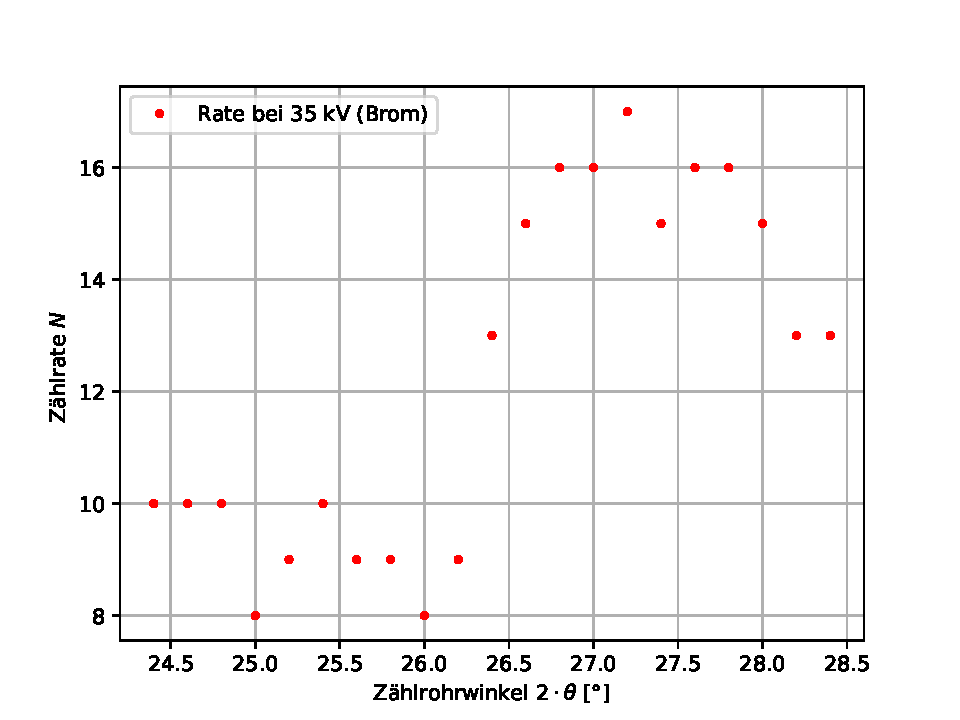
\includegraphics[height=8cm]{Auswertung/Brom.pdf}
    \caption{Absorptionsspektrum für Brom.}
    \label{fig:Brom}
\end{figure}

Zur Bestimmung der K-Kante wird der Winkel bei der Hälfte der maximalen Zählrate verwendet.
Für Brom wird dabei ein Winkel und eine dazugheörige Energie von
\begin{equation}
    \theta = \SI{13,2}{°} \qquad \text{und} \qquad E = \SI{13,507}{keV}  \notag
\end{equation}
bestimmt.
Im Vergleich zu dem theoretisch bestimmten Wert von $E_\text{theo} = \SI{13,470}{keV}$ ergibt sich eine Abweichung von $0,3\%$.
Mittels Gleichung \ref{eqn:ab} wird die Abschirmkonstante mit $z = 35$
\begin{equation}
    \sigma_1 = 3,170  \notag
\end{equation}
bestimmt, wobei der theoretische Wert $\sigma_\text{1,theo} = 3,830$ beträgt und der Wert somit eine Abweichung von $17,2 \%$ hat.

\subsubsection{Moseleysches-Gesetz}
Das Moseleysche Gesetz besagt, dass sich die Absorptionsenergie der K-Kante $E_K$ proportional zum Quadrat der Kernladungszahl verhält.
Dabei werden die gemessenen Werte für Gallium, Zink, Zirkonium und Brom in einem $\sqrt{E_K}$-$z$-Diagramm in Abbildung \ref{fig:moseley} aufgetragen.

\begin{figure}[h!]
    \centering
    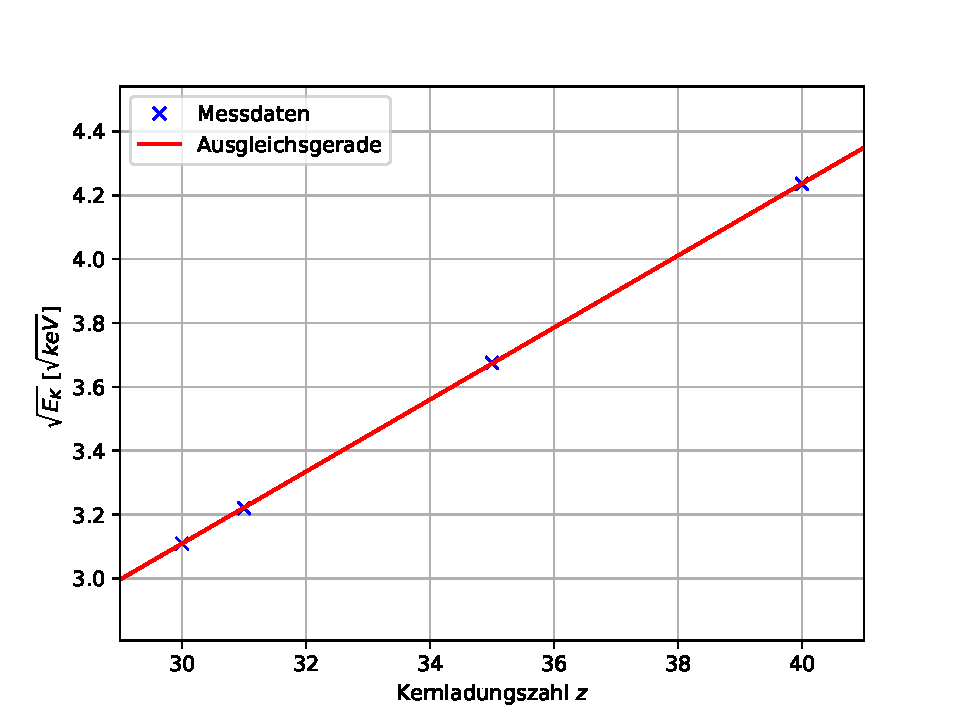
\includegraphics[height=8cm]{Auswertung/Moseley.pdf}
    \caption{Auftragung der Kernladungszahl gegen die Wurzel der Energie der K-Kanten.}
    \label{fig:moseley}
\end{figure}

Die lineare Regression nach 
\begin{equation}
    y = m \cdot x + b
\end{equation}
liefert die Parameter
\begin{equation}
    m = \SI{0.113}{keV^{\frac{1}{2}}}  \qquad \text{und}   \qquad b = \SI{-0,272 \pm 8.110}{keV^{\frac{1}{2}}}. \notag
\end{equation}.
Dabei ist die $R_\infty = m^{2}$ und es ergibt sich
\begin{equation}
    R_\infty = \SI{12,769}{eV}
\end{equation}
und zum Literaturwert der Rydbergenergie $R_\text{$\infty$,Lit} = \SI{13,6}{eV}$ damit eine Abweichung von $6,2 \%$
\subsubsection{Wismutabsober}
Bei Wismut wird die Absorptionsenergie der L-Kante untersucht.
Dabei werden die Winkel
\begin{equation}
    \theta_2 = \SI{11,5}{°} \qquad \text{und} \qquad \theta_3 = \SI{13,5}{°}  \notag
\end{equation}
für die beiden L-Kanten aus dem Absorptionsspektrum in Abbildung \ref{fig:wismut} abgelesen.

\begin{figure}[H]
    \centering
    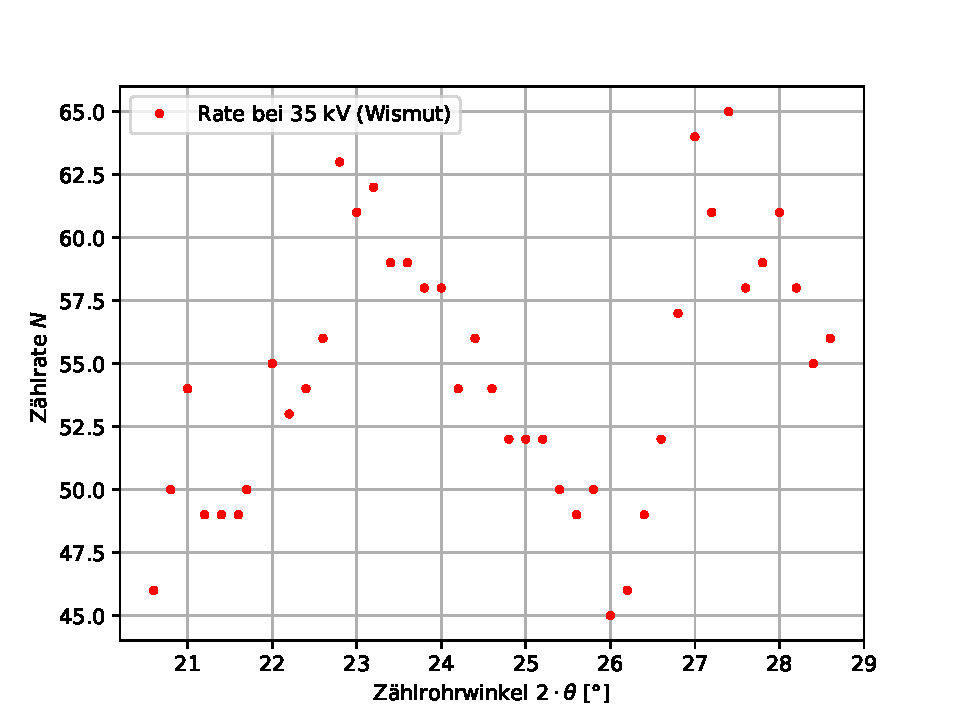
\includegraphics[height=8cm]{Auswertung/Wismut.pdf}
    \caption{Absorptionsspektrum für Wismut.}
    \label{fig:wismut}
\end{figure}

Daraus ergeben sich Energien von
\begin{equation}
    E_1 = \SI{15,470}{keV}  \qquad \text{und}   \qquad E_2 = \SI{13,212}{keV},  \notag
\end{equation}
aus denen sich die Abschirmkonstante bestimmen lässt.
Die L-Kanten haben zu den Literaturwerten
\begin{equation}
    E_\text{1,Lit} = \SI{15,719}{keV} \qquad \text{und} \qquad E_\text{2,Lit} = \SI{13,427}{keV}
\end{equation}
Abweichungen von jeweils $1,6 \%$.
Es resultiert eine Energiedifferenz der L-Kanten von
\begin{equation}
    \Delta E_L = \SI{2,268}{keV}.   \notag
\end{equation}
Der Literaturwert beträgt $E_\text{L,theo} = \SI{2,298}{keV}$ \cite{2} und der experimentell ermittelte Wert hat somit eine Abweichung von $1,3 \%$.
Mittels Gleichung \ref{eq:4} und einer Kernladungszahl von $z = 83$ wird die Abschirmkonstante auf
\begin{equation}
     \sigma_L = 3,766   \notag
\end{equation}
bestimmt.

\subsection{Tabellen}

\begin{table} [H]
    \label{tab:Bragg}
  \begin{minipage}{0.5\textwidth}
    \begin{tabular}{c|c}
      \textbf{Zählrohrwinkel $2 \cdot \theta$ $[°]$} & \textbf{Zählrate $N$}\\
      \hline
      26,0   & 47,0 \\
      26,1   & 50,0 \\
      26,2	 & 48,0 \\
      26,3	 & 50,0 \\
      26,4	 & 47,0 \\
      26,5	 & 54,0 \\
      26,6	 & 54,0 \\
      26,7	 & 51,0 \\
      26,8	 & 49,0 \\
      26,9	 & 55,0 \\
      27,0	 & 54,0 \\
      27,1	 & 56,0 \\
      27,2	 & 61,0 \\
      27,3	 & 63,0 \\
      27,4	 & 70,0 \\
      27,5	 & 82,0 \\
      27,6	 & 88,0 \\
      27,7	 & 87,0 \\
      27,8	 & 102,0 \\
      27,9	 & 120,0 \\
      28,0	 & 125,0
    \end{tabular}
  \end{minipage}
    \hfill
  \begin{minipage}{0.5\textwidth} 
    \begin{tabular}{c|c}
        \textbf{Zählrohrwinkel $2 \cdot \theta$ $[°]$} & \textbf{Zählrate $N$}\\
      \hline
      28,1	 & 131,0 \\
      28,2	 & 147,0 \\
      28,3	 & 157,0 \\
      28,4	 & 174,0 \\
      28,5	 & 186,0 \\
      28,6	 & 199,0 \\
      28,7	 & 198,0 \\
      28,8	 & 199,0 \\
      28,9	 & 194,0 \\
      29,0	 & 185,0 \\
      29,1	 & 179,0 \\
      29,2	 & 168,0 \\
      29,3	 & 162,0 \\
      29,4	 & 162,0 \\
      29,5	 & 142,0 \\
      29,6	 & 130,0 \\
      29,7	 & 118,0 \\
      29,8	 & 108,0 \\
      29,9	 & 83,0 \\
      30,0	 & 76,0 \\
        &
    \end{tabular}
  \end{minipage}
    \caption{Messwerte zur Überprüfung der Bragg-Bedingung.}
  \end{table}

  \begin{table}[H]
  \begin{minipage}[c]{0.5\textwidth}
    \label{tab:gallium}
    \begin{tabular}{c|c}
      \textbf{Zählrohwinkel $2 \cdot \theta$ $[°]$} & \textbf{Zählrate $N$}\\
      \hline
      32,5	& 36,0 \\
      32,8	& 38,0 \\
      33,0	& 37,0 \\
      33,2	& 38,0 \\
      33,4	& 37,0 \\
      33,6	& 35,0 \\
      33,8	& 36,0 \\
      34,0	& 35,0 \\
      34,2	& 33,0 \\
      34,4	& 39,0 \\
      34,5	& 44,0 \\
      34,8	& 49,0 \\
      35,0	& 54,0 \\
      35,2	& 53,0 \\
      35,4	& 55,0 \\
      35,5	& 47,0 \\
      35,8	& 48,0 \\
      36,0	& 52,0 \\
      36,2	& 49,0 \\
      36,4	& 46,0 \\
      36,5	& 49,0
    \end{tabular}
    \captionsetup{width=7cm}
    \caption{Messung der Zählrate bei Gallium für verschiedene Zählrohrwinkel.}
  \end{minipage}
    \hfill
  \begin{minipage}[c]{0.5\textwidth}
    \label{tab:zink}
    \begin{tabular}{c|c}
        \textbf{Zählrohrwinkel $2 \cdot \theta$ $[°]$} & \textbf{Zählrate $N$}\\
      \hline
      35,0	& 43,0 \\
      35,2	& 43,0 \\
      35,4	& 42,0 \\
      35,5	& 40,0 \\
      35,8	& 40,0 \\
      36,0	& 41,0 \\
      36,2	& 41,0 \\
      36,4	& 39,0 \\
      36,5	& 40,0 \\
      36,8	& 40,0 \\
      37,0	& 42,0 \\
      37,2	& 49,0 \\
      37,4	& 58,0 \\
      37,5	& 59,0 \\
      37,8	& 59,0 \\
      38,0	& 61,0 \\
      38,2	& 61,0 \\
      38,4	& 61,0 \\
      38,6	& 64,0 \\
      38,8	& 66,0 \\
      39,0	& 66,0
    \end{tabular}
    \captionsetup{width=7cm}
    \caption{Messung der Zählrate bei Zink für verschiedene Zählrohrwinkel.}
  \end{minipage}
\end{table}

\begin{table}[H]
\begin{minipage}[c]{0.5\textwidth}
    \label{tab:zirkonium}
  \begin{tabular}{c|c}
    \textbf{Zählrohrwinkel $2 \cdot \theta$ $[°]$} & \textbf{Zählrate $N$}\\
    \hline
    17,6	& 64,0 \\
    17,7	& 63,0 \\
    18,0	& 64,0 \\
    18,2	& 64,0 \\
    18,4	& 59,0 \\
    18,6	& 60,0 \\
    18,8	& 59,0 \\
    19,0	& 55,0 \\
    19,2	& 60,0 \\
    19,4	& 64,0 \\
    19,6	& 73,0 \\
    19,8	& 86,0 \\
    20,0	& 95,0 \\
    20,2	& 99,0 \\
    20,4	& 101,0 \\
    20,6	& 97,0 \\
    20,8	& 95,0 \\
    21,0	& 96,0 \\
    21,2	& 94,0 \\
    21,4	& 97,0 \\
    21,6	& 97,0
  \end{tabular}
  \captionsetup{width=7cm}
  \caption{Messung der Zählrate bei Zirkonium für verschiedene Zählrohrwinkel.}
\end{minipage}
  \hfill
\begin{minipage}[c]{0.4\textwidth}
    \label{tab:brom}
  \begin{tabular}{c|c}
    \textbf{Zählrohrwinkel $2 \cdot \theta$ $[°]$} & \textbf{Zählrate $N$}\\
    \hline
    24,4	& 10,0 \\
    24,6	& 10,0 \\
    24,8	& 10,0 \\
    25,0	& 8,0 \\
    25,2	& 9,0 \\
    25,4	& 10,0 \\
    25,6	& 9,0 \\
    25,8	& 9,0 \\
    26,0	& 8,0 \\
    26,2	& 9,0 \\
    26,4	& 13,0 \\
    26,6	& 15,0 \\
    26,8	& 16,0 \\
    27,0	& 16,0 \\
    27,2	& 17,0 \\
    27,4	& 15,0 \\
    27,6	& 16,0 \\
    27,8	& 16,0 \\
    28,0	& 15,0 \\
    28,2	& 13,0 \\
    28,4	& 13,0
  \end{tabular}
  \captionsetup{width=7cm}
  \caption{Messung der Zählrate bei Brom für verschiedene Zählrohrwinkel.}
\end{minipage}
\end{table}


\begin{table}[H]
  \begin{center}
    \label{tab:wismut}
    \begin{tabular}{c|c} 
        \textbf{Zählrohrwinkel $2 \cdot \theta$ $[°]$} & \textbf{Zählrate $N$}\\
      \hline
      20,6	& 46,0 \\
      20,8	& 50,0 \\
      21,0	& 54,0 \\
      21,2	& 49,0 \\
      21,4	& 49,0 \\
      21,6	& 49,0 \\
      21,7	& 50,0 \\
      22,0	& 55,0 \\
      22,2	& 53,0 \\
      22,4	& 54,0 \\
      22,6	& 56,0 \\
      22,8	& 63,0 \\
      23,0	& 61,0 \\
      23,2	& 62,0 \\
      23,4	& 59,0 \\
      23,6	& 59,0 \\
      23,8	& 58,0 \\
      24,0	& 58,0 \\
      24,2	& 54,0 \\
      24,4	& 56,0 \\
      24,6	& 54,0 \\
      24,8	& 52,0 \\
      25,0	& 52,0 \\
      25,2	& 52,0 \\
      25,4	& 50,0 \\
      25,6	& 49,0 \\
      25,8	& 50,0 \\
      26,0	& 45,0 \\
      26,2	& 46,0 \\
      26,4	& 49,0 \\
      26,6	& 52,0 \\
      26,8	& 57,0 \\
      27,0	& 64,0 \\
      27,2	& 61,0 \\
      27,4	& 65,0 \\
      27,6	& 58,0 \\
      27,8	& 59,0 \\
      28,0	& 61,0 \\
      28,2	& 58,0 \\
      28,4	& 55,0 \\
      28,6	& 56,0
    \end{tabular}
    \caption{Messung der Zählrate bei Wismut für verschiedene Zählrohrwinkel.}
  \end{center}
\end{table}
